%\subsection{Heat Pump}
\subsubsection{Heat Pump}

A heat pump can be modeled in several ways. A straightforward approach is to reduce the heat pump to two \textsf{FixedNode} objects, external to the building system. These nodes represent the evaporator and condensor \emph{exit} temperatures $T_{evap}$ and $T_{cond}$. In case of a air-water heatpump, $T_{evap}$ can be approximated with the instantaneous outdoor (ambient) temperature from the weather conditions. For a heat pump with a liquid heat source this will be the source temperature, in any cases a ground source. $T_{cond}$ can be derived from a heating curve ($T_{cond}$ vs. $T_{outdoor}$) or from a heat pump functional model.

The elements of the heat pump model are:

\begin{itemize}
	\item a "hot" condensor node $T_{cond}$. This is a node of type \textsf{FixedNode} or \textsf{CapacityNode}(see section \ref{sec:capnode}).
	\item a "cold" condensor node $T_{return}$. This is a node of type \textsf{FixedNode} (see section \ref{sec:fixnode}), with a variable temperature, but no heat capacity.
	\item an "ambient" temperature $T_{evap}$ at the evaporator side of the heat pump \textit{i.e.} the "outdoor" node of the building in the model.
	\item a \textsf{Flow} object with a \textsf{node\_list} starting at the hot node, passing through \textit{e.g.} a buffer vessel. There, (part of) the thermal energy is stored. Via the bottom layer of the vessel the flow returns to the cold condensor node.  Thermal power is added by the heat pump, to increase the temperature of the water from $T_{return}$ to $T_{cond}$. The flow object has an attribute $F_{hp}$ which equals the magnitude of the thermal heat transfer in $[W/K]$.
	\item the instantaneous thermal power $\dot{q}_{hp}$, delivered by the heat pump to the condensor flow circuit and the buffer vessel. Equals $F_{hp} \cdot (T_{cond} - T_{return})$. The maximal value of $\dot{q}_{hp}$ is a function of of $T_{cond}$ and $T_{evap}$.
	\item the instantaneous electric power $P_{el}$. Usually, a heat pump has characteristic curves, giving the \emph{coefficient of performance (COP)} as a function of $T_{cond}$ and $T_{evap}$. COP equals $\dot{q}_{hp}/P_{el}$. 
\end{itemize} 

\begin{figure}[h!]
	\begin{center}
		\begin{circuitikz}
			\ctikzset{bipoles/thickness=3}
			\draw (8,0)
			node[color=darkgreen, circ, label={[darkgreen]above:$T_{bottom}$}]{}
			to[R,R=$R_{mid,bot}$] (8,4) 
			node[color=darkgreen, circ, label={[darkgreen]above:$T_{mid}$}]{}
			to[R,R=$R_{top,mid}$, -*] (8,8)
			node[color=darkgreen, circ, label={[darkgreen]above:$T_{top}$}]{};
			\draw (8,0)
			node[color=darkgreen, circ, label={[darkgreen]above:$T_{bottom}$}]{}
			to[R,R=$R_{mid,bot}$] (8,4) 
			node[color=darkgreen, circ, label={[darkgreen]above:$T_{mid}$}]{}
			to[R,R=$R_{top,mid}$, -*] (8,8)
			node[color=darkgreen, circ, label={[darkgreen]above:$T_{top}$}]{};
			\draw (8.5,0)
			to [short] (8.5,8)
			to [short] (11,8)
			to [short] (11,5)
			to [short] (12,5)
			node[color=red, circ, label={[red]above:$T_{feed}$}]{}
			to [short, *-*] (12,3)
			node[color=blue, circ, label={[blue]above:$T_{return}$}]{}
			to [short] (11,3)
			to [short] (11,0)
			to [short] (8.5,0)
			(16,4) to[amp, label=$\dot{Q}_{heat pump}$] ++(-4,0);
		\end{circuitikz}
		\caption{Heat pump model.}
		\label{fig:hpmodel}
	\end{center}
\end{figure}

In Fig.~\ref{fig:hpmodel} a heat pump is shown with its nodes, surroundings and a buffer vessel for generating a supply and return flow. The heat pump will deliver its thermal power via an internal heat exchanger from the condensor side to a liquid heat carrier (water) in a buffer vessel. For the liquid medium, the following equation holds:

\begin{equation}\color{blue}
	\label{eq:hpflow}
	\begin{aligned}
		F_{hp} &= \dot{f} \cdot \rho \cdot c_w  &= \dot{m} \cdot c_w 
	\end{aligned}
\end{equation}

where: \\
$\rho$ is the density of the medium in $[kg/m^3]$ \\
$c_w$ is the specific heat capacity of water: $4.2 \cdot 10^3 J/(kg \cdot K)$ \\
$\dot{f}$ is the liquid volume flow in $[m^3/s]$ \\
$\dot{m}$ is the liquid mass flow in $[kg/s]$ \\

There are a few options for the connection of the buffer vessel:

\subsubsection{4-way connection}

The most straightforward connection method is a 4-way connection, as shown in Figure~\ref{fig:4way}. The heat source (heat pump) thermally loads the buffer vessel in the top layer. The thermal demand is also taken from the top layer. For low-temperature radiators or a floor heating circuit there is a mixing valve that short circuits feed and return water, to provide an adjustable temperature heat source for the delivery system. The remaining return flow from the delivery system is passed back to the bottom layer of the buffer vessel. The heat source return water is also taken from the bottom layer.

\begin{figure}[H]
	\centering
	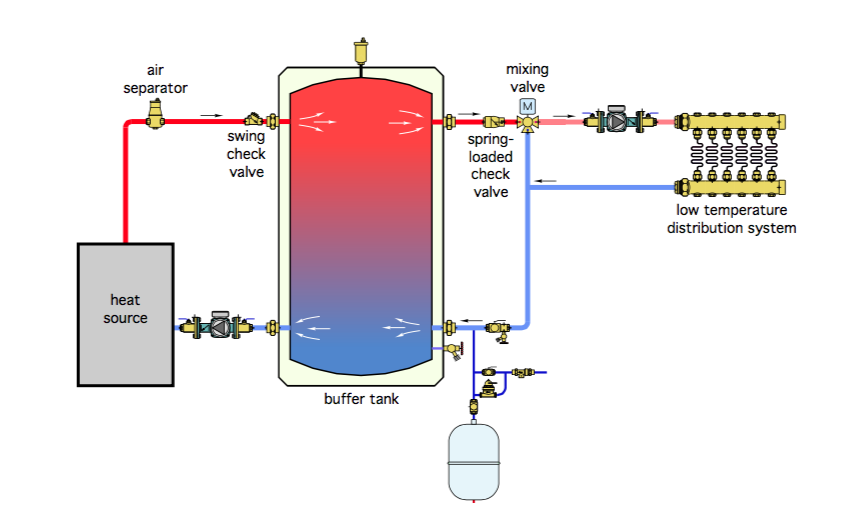
\includegraphics[width=0.7\columnwidth]{Figures/4-way buffer connection}
	\caption[Short title]{4-way connection of stratified buffer vessel.}
	\label{fig:4way}
\end{figure} 

\begin{figure}[H]
	\centering
	\begin{subfigure}[b]{0.45\textwidth}
		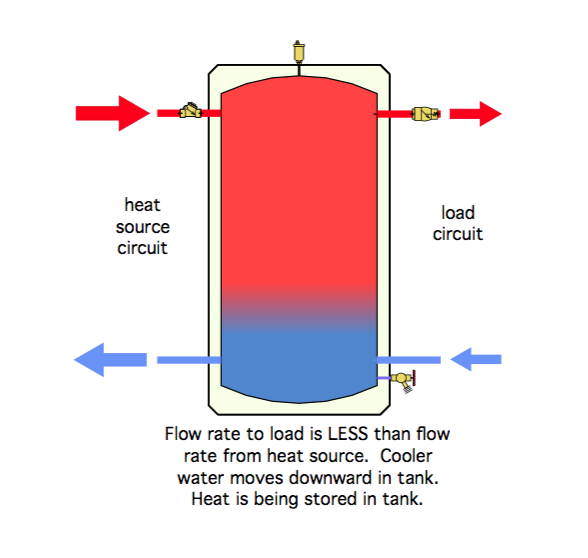
\includegraphics[width=\textwidth]{Figures/4-way buffer loaded}
		\caption{Buffer vessel loading...}
		\label{fig:4way_loaded}
	\end{subfigure}
	\hfill
	\begin{subfigure}[b]{0.45\textwidth}
		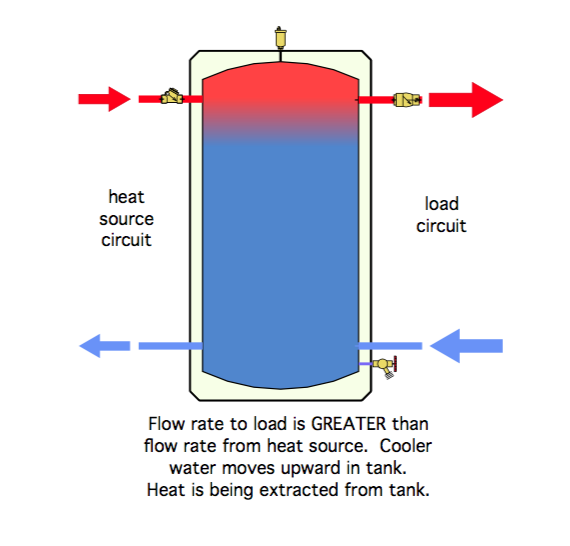
\includegraphics[width=\textwidth]{Figures/4-way buffer unloading}
		\caption{Buffer vessel unloading...}
		\label{fig:4way_unloading}
	\end{subfigure}
	\caption{Stratified buffer vessel dynamics.}
	\label{fig:4way_dynamics}
\end{figure}

\subsubsection{2-way connection}

\begin{figure}[H]
	\centering
	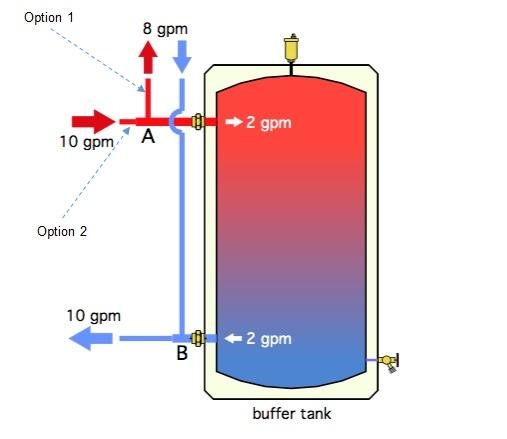
\includegraphics[width=0.5\columnwidth]{Figures/2-way buffer connection}
	\caption[Short title]{2-way connection of stratified buffer vessel.}
	\label{fig:2way}
\end{figure} 


The \textsf{HeatPump} class in Python encapsulates the attributes above and the calculation of $F_{hp}$. The methods of this class are:
\begin{itemize}
	\item \textsf{\_\_init\_\_}: initializes the class members. Members starting with \_\_* are private members.
\end{itemize}

\lstinputlisting[label=lst:Radiator, linerange={20-35}, 
caption={HeatPump class}] 
{../../housemodel/sourcesink/heatpumps/heatpumpnew.py}

\begin{itemize}
	\item \textsf{from\_dict}. This method operates as an "overloaded" constructor, reading from a Python \textsf{dictionary}.
\end{itemize}

\lstinputlisting[label=lst:Radiator, linerange={37-41}, 
caption={Heatpump constructor from dictionary}] 
{../../housemodel/sourcesink/heatpumps/heatpumpnew.py}

\begin{itemize}
	\item \textsf{set\_cal\_val}: set the values of calibration constants $c_0$, $c_1$ and $c_2$ from NTA8800:2022, Appendix Q.
	\item \textsf{set\_A2W35}: set COP and $P_{max}$ for an ambient temperature of $2~ \degC$ and a condensor delivery temperature of  $35~\degC$.
\end{itemize}

\lstinputlisting[label=lst:Radiator, linerange={46-52}, 
caption={Heatpump calibration methods}] 
{../../housemodel/sourcesink/heatpumps/heatpumpnew.py}

Calculations for solving the vector $\mathbf{x} = [\text{COP} \quad P_{max}]^T$ are performed in the method \textsf{update}. This method interpolates the calibration curves for COP and $P_{max}$ for a given $T_{amb}$ and $T_{cond}$. 

\lstinputlisting[label=lst:lmtd, linerange={54-73}, 
caption={\textsf{update} method}]
{../../housemodel/sourcesink/heatpumps/heatpumpnew.py}

\newpage
